\documentclass[landscape]{article}
\usepackage[pdftex]{graphicx,color,rotating}
\pagestyle{empty}
\oddsidemargin  -0.5 in
\evensidemargin -0.5 in
\headheight     0 in
\topmargin      -1 in
\textheight     7.7 in
\textwidth      10 in
\begin{document}
\Large
\renewcommand{\labelitemi}{-}
\setlength{\parindent}{0 cm}

\mbox{ }

\vspace{0.5 cm}

\begin{center}\fbox{\begin{minipage}{0.75\linewidth}
    A quick quick explaination:

    $\Upsilon$ decays were split into five classes, and mode-by-mode
    efficiencies are plotted on each of five pages.  A sixth page
    shows $\tau^+\tau^-$ events split up by how they decay.  On the
    last page are aggregate efficiencies of all events, with all the
    proper correlations taken into account.

    Talk to you Wednesday!
    \end{minipage}}
\end{center}

\vspace{1 cm}

A (not-actually) quick explaination:

\vspace{0.2 cm} \hspace{0.2 cm} This document illustrates the efficiency of these cuts:
\begin{center}
  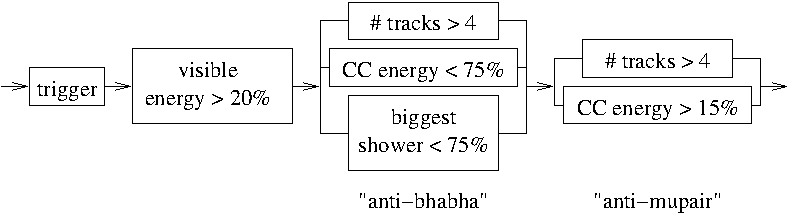
\includegraphics[width=0.5\linewidth]{analysismc_cuts.pdf}
\end{center}
as a function of decay mode.  Since there are N$^{\mbox{???}}$ different
possible decay trees for inclusive $\Upsilon \to$ anything, the decay
trees are divided into one of these classes:

\begin{center}
  \begin{tabular}{c | c | c | c | c | c}
    $b\bar{b}$ decays to\ldots & $X\,ggg$ or $X\,gg$ & $X\,gg\gamma$ & $X\,e^+e^-$ & $X\,\mu^+\mu^-$ & $X\,\tau^+\tau^-$ \\\hline
    PHOTOS was used & & & & & \\
    in the $b\bar{b}$ decay & & & & & \\\hline
    PHOTOS wasn't used & & & & & \\
  \end{tabular}
\end{center}

\vspace{0.2 cm} \hspace{0.2 cm} Each of these classes will be presented on a separate page.  For the
$\Upsilon(1S)$, there is only one way to decay to the specified mode
(two in the case of PHOTOS, as there may be one or two photons), but
for the $\Upsilon(2S)$ and $\Upsilon(3S)$, there are many cascade
chains to get to the specified final state; the efficiency of each of
these subclasses will be determined, plotted, and used for later
calculations.

\vspace{1.4 cm} \hspace{0.2 cm} These subclasses are singletons for $e^+e^-$ and $\mu^+\mu^-$ but very
large sets for $ggg$, $gg\gamma$, and $\tau^+\tau^-$.  Breaking up
$ggg$ and $gg\gamma$ would be difficult, since they can decay to
nearly anything.  Fortunately, it's unnecessary: $ggg$ are highly
efficient and the efficiency of $gg\gamma$ depends mostly on the
spectrum of the high-energy photon.  But $\tau^+\tau^-$ have
widely-varying efficiencies which depend strongly on the decay
topology, so I split these up into 111 sub-subclasses: the top ten
$\tau$ decays + 1 ``everything else'', all squared to let the two
sides of the event decay independently.

\vspace{1.4 cm} \hspace{0.2 cm} At the bottom of each page, I calculate the aggregate efficiency for
each class, combining subclasses (and sub-subclasses) according to
their PDG branching fractions, which I vary according to their PDG
uncertainties.  This calculation is done with a toy Monte Carlo which
takes all correlations into account: leptonic branching fractions are
equal, and $\tau^-$ decays are equal to their conjugate $\tau^+$
decays.  All other inputs were determined using independent data and
are therefore varied independently.

\vspace{1.4 cm} \hspace{0.2 cm} PHOTOS-ified modes couldn't be varied this way, since PDG branching
fractions integrate over soft photons.  So PHOTOS's mode-by-mode
branching fractions were taken directly from the MC--- {\it not}
fluctuated.  The efficiencies listed on the bottoms of each page have
non-PHOTOfied and PHOTOfied modes combined, and just to tune this
effect, I fluctuated the overall normalization of PHOTOfied to
non-PHOTOfied modes by 30\%.  (We can change that later.)
Non-PHOTOfied modes are usually far more numerous than PHOTOfied ones,
so it's reasonable to give the non-PHOTOfied ones more attention.
(Only for final-state leptons are the PHOTOfied modes actually
significant--- for these, I had to adjust my PDG leptonic branching
fraction to avoid double-counting.  This is a detail.)

\vspace{1.4 cm} \hspace{0.2 cm} The last variable I fluctuated was the ratio of events that decay to
$ggg$ versus those that decay to $gg\gamma$.  This is a QED
calculation, but just because it doesn't hurt, I varied it up and down
33\%.  (The nominal value is 0.03 $gg\gamma$ to $ggg$.)  This relates
two distinct classes (two pages), so it only comes into the
calculation of ``branching fraction to this set of modes'' on the
bottom-right of the page.  It's the {\color{blue} blue} error.  (The
black error that preceeds it comes from PDG uncertainties.)

\vspace{1.4 cm} \hspace{0.2 cm} On the last page, I put everything together to calculate the total
efficiency and hadronic efficiency of these cuts.  To get all the
correlations right, I did it in one big toy MC, combining all classes.
I still vary PDG uncertainties, PHOTOSification probability, and
$\mathcal{B}(\frac{gg\gamma}{ggg})$, and often the overall
uncertainties are less than what they would seem from the individual
pages, since there are many large correlations.  I repeated each
calculation using Istvan's 6/15/04 $\mathcal{B}_{\mu\mu}$.

\vspace{1.4 cm} \hspace{0.2 cm} (Incidentally, this hadronic efficiency is really the hadronic
efficiency, defined as the rest of the world defines it: so
$\Upsilon(3S) \to \pi^0 \pi^0 \Upsilon(1S)$, $\Upsilon(1S) \to e^+e^-$
is counted as hadronic, and $\Upsilon(1S) \to \tau^+\tau^- \to$ 10
tracks is counted as leptonic.  We get the expected behavior that
hadronic efficiencies are better known than total efficiencies.)

\vspace{1.4 cm} \hspace{0.2 cm} (Also on the last page, I didn't break $\tau^+\tau^-$ up into
sub-subclasses because this didn't make much difference: the top ten
decay modes of the $\tau$ are all known to better than 1\% of the
total $\tau$ width, so even though their efficiencies depend very much
on mode, the modes are properly modelled in the Monte Carlo.)

\vspace{1.4 cm} \hspace{0.2 cm} This work is the result of a lot of internal cross-checks (that's why
it's so late), and I claim that I can explain any relationship in the
results.  We'll see!

\pagebreak

\begin{tabular}{p{0.02\linewidth} p{0.95\linewidth}}
  \begin{minipage}{\linewidth}
    \mbox{\hspace{0.3 cm} \begin{rotate}{90}
	\hspace{-3 cm} Occurrences in MC sample
    \end{rotate}}
  \end{minipage} &
  \begin{minipage}{\linewidth}
    \hspace{-0.5 cm} 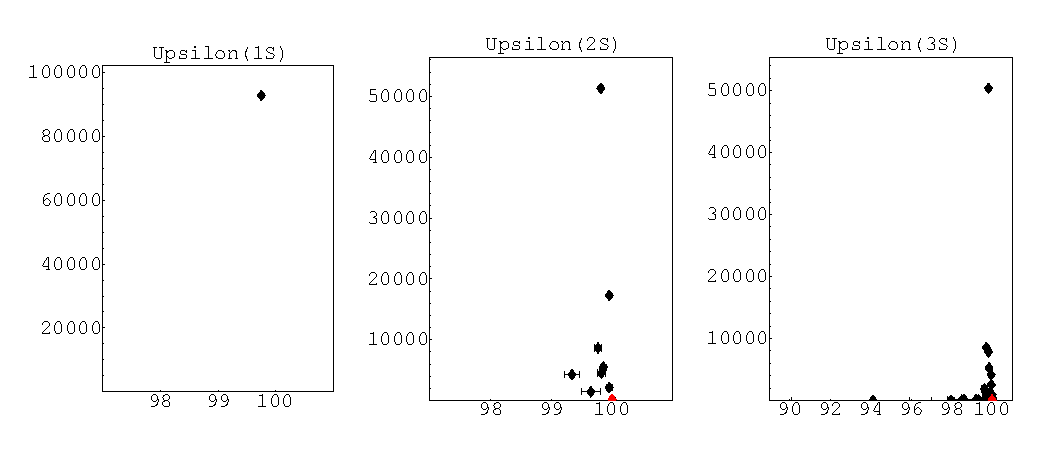
\includegraphics[width=\linewidth]{decayplot_glue.pdf}
  \end{minipage} \\
  & \begin{minipage}{\linewidth}
    \begin{center}
      \vspace{-1.3 cm}
      Cut efficiency for each $\Upsilon \to \ldots \to$ gluons mode {\color{red} (red modes are from PHOTOS)}
    \end{center}
  \end{minipage}
\end{tabular}

\begin{center}
  \begin{tabular}{c | c c c c | c}
    \hline\hline
    & & & & & \\
    \begin{minipage}{3 cm} \begin{center} Resonance \end{center} \end{minipage} &
    \begin{minipage}{2 cm} \begin{center} Cut efficiency \end{center} \end{minipage} &
    \begin{minipage}{2 cm} \begin{center} Statisical Error \end{center} \end{minipage} &
    \begin{minipage}{4 cm} \begin{center} Variation with PDG mode uncertainties \end{center} \end{minipage} &
    \begin{minipage}{4 cm} \begin{center} Variation with fluctuating PHOTOS 30\% \end{center} \end{minipage} &
    \begin{minipage}{3 cm} \begin{center} Branching fraction to this set of modes \end{center} \end{minipage} \\
    & & & & & \\\hline
    & & & & & \\
    $\Upsilon(1S)$ & 99.752\% & $\pm$ 0.016 & $\pm$ 0 & $\pm$ 0 & 89.783\% $\pm$ 0.084 {\color{blue} $\pm$ 0.93} \\
    & & & & & \\
    $\Upsilon(2S)$ & 99.821\% & $\pm$ 0.014 & $\pm$ 0.0034 & $\pm$ 0.0001 & 91.48\% $\pm$ 0.26 {\color{blue} $\pm$ 0.81} \\
    & & & & & \\
    $\Upsilon(3S)$ & 99.823\% & $\pm$ 0.014 & $\pm$ 0.0017 & $\pm$ 0.0001 & 90.91\% $\pm$ 0.30 {\color{blue} $\pm$ 0.70} \\
    & & & & & \\\hline\hline
  \end{tabular}
\end{center}

\pagebreak

\begin{tabular}{p{0.02\linewidth} p{0.95\linewidth}}
  \begin{minipage}{\linewidth}
    \mbox{\hspace{0.3 cm} \begin{rotate}{90}
	\hspace{-3 cm} Occurrences in MC sample
    \end{rotate}}
  \end{minipage} &
  \begin{minipage}{\linewidth}
    \hspace{-0.5 cm} 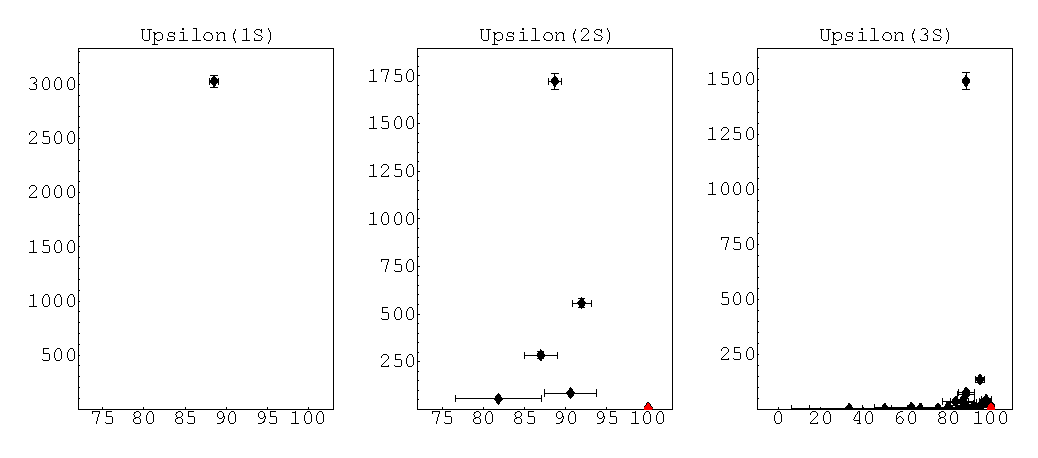
\includegraphics[width=\linewidth]{decayplot_ggpho.pdf}
  \end{minipage} \\
  & \begin{minipage}{\linewidth}
    \begin{center}
      \vspace{-1.1 cm}
      Cut efficiency for each $\Upsilon \to \ldots \to gg\gamma$ mode {\color{red} (red modes are from PHOTOS)}
    \end{center}
  \end{minipage}
\end{tabular}

\begin{center}
  \begin{tabular}{c | c c c c | c}
    \hline\hline
    & & & & & \\
    \begin{minipage}{3 cm} \begin{center} Resonance \end{center} \end{minipage} &
    \begin{minipage}{2 cm} \begin{center} Cut efficiency \end{center} \end{minipage} &
    \begin{minipage}{2 cm} \begin{center} Statisical Error \end{center} \end{minipage} &
    \begin{minipage}{4 cm} \begin{center} Variation with PDG mode uncertainties \end{center} \end{minipage} &
    \begin{minipage}{4 cm} \begin{center} Variation with fluctuating PHOTOS 30\% \end{center} \end{minipage} &
    \begin{minipage}{3 cm} \begin{center} Branching fraction to this set of modes \end{center} \end{minipage} \\
    & & & & & \\\hline
    & & & & & \\
    $\Upsilon(1S)$ & 88.51\% & $\pm$ 0.58 & $\pm$ 0 & $\pm$ 0 & 2.7769\% $\pm$ 0.0026 {\color{blue} $\pm$ 0.93} \\
    & & & & & \\
    $\Upsilon(2S)$ & 89.16\% & $\pm$ 0.60 & $\pm$ 0.042 & $\pm$ 0.0024 & 2.410\% $\pm$ 0.032 {\color{blue} $\pm$ 0.80} \\
    & & & & & \\
    $\Upsilon(3S)$ & 89.18\% & $\pm$ 0.68 & $\pm$ 0.091 & $\pm$ 0.014 & 2.091\% $\pm$ 0.035 {\color{blue} $\pm$ 0.70} \\
    & & & & & \\\hline\hline
  \end{tabular}
\end{center}

\pagebreak

\begin{tabular}{p{0.02\linewidth} p{0.95\linewidth}}
  \begin{minipage}{\linewidth}
    \mbox{\hspace{0.3 cm} \begin{rotate}{90}
	\hspace{-3 cm} Occurrences in MC sample
    \end{rotate}}
  \end{minipage} &
  \begin{minipage}{\linewidth}
    \hspace{-0.5 cm} 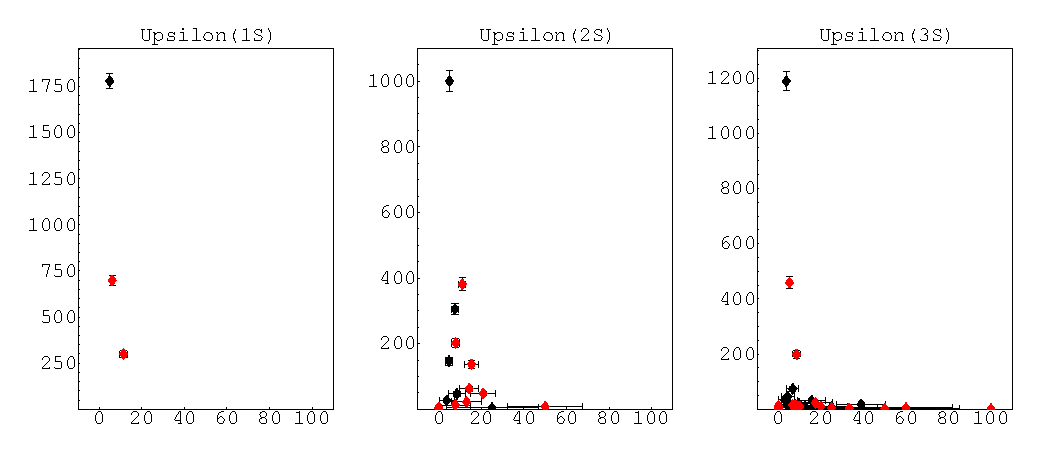
\includegraphics[width=\linewidth]{decayplot_ee.pdf}
  \end{minipage} \\
  & \begin{minipage}{\linewidth}
    \begin{center}
      \vspace{-1.1 cm}
      Cut efficiency for each $\Upsilon \to \ldots \to X e^+e^-$ mode {\color{red} (red modes are from PHOTOS)}
    \end{center}
  \end{minipage}
\end{tabular}

\begin{center}
  \begin{tabular}{c | c c c c | c}
    \hline\hline
    & & & & & \\
    \begin{minipage}{3 cm} \begin{center} Resonance \end{center} \end{minipage} &
    \begin{minipage}{2 cm} \begin{center} Cut efficiency \end{center} \end{minipage} &
    \begin{minipage}{2 cm} \begin{center} Statisical Error \end{center} \end{minipage} &
    \begin{minipage}{4 cm} \begin{center} Variation with PDG mode uncertainties \end{center} \end{minipage} &
    \begin{minipage}{4 cm} \begin{center} Variation with fluctuating PHOTOS 30\% \end{center} \end{minipage} &
    \begin{minipage}{3 cm} \begin{center} Branching fraction to this set of modes \end{center} \end{minipage} \\
    & & & & & \\\hline
    & & & & & \\
    $\Upsilon(1S)$ & 5.87\% & $\pm$ 0.63 & $\pm$ 0 & $\pm$ 0.29 & 2.479\% $\pm$ 0.050 \\
    & & & & & \\
    $\Upsilon(2S)$ & 7.95\% & $\pm$ 0.77 & $\pm$ 0.061 & $\pm$ 0.67 & 2.04\% $\pm$ 0.14 \\
    & & & & & \\
    $\Upsilon(3S)$ & 5.48\% & $\pm$ 0.67 & $\pm$ 0.11 & $\pm$ 0.28 & 2.30\% $\pm$ 0.17 \\
    & & & & & \\\hline\hline
  \end{tabular}
\end{center}

\pagebreak

\begin{tabular}{p{0.02\linewidth} p{0.95\linewidth}}
  \begin{minipage}{\linewidth}
    \mbox{\hspace{0.3 cm} \begin{rotate}{90}
	\hspace{-3 cm} Occurrences in MC sample
    \end{rotate}}
  \end{minipage} &
  \begin{minipage}{\linewidth}
    \hspace{-0.5 cm} 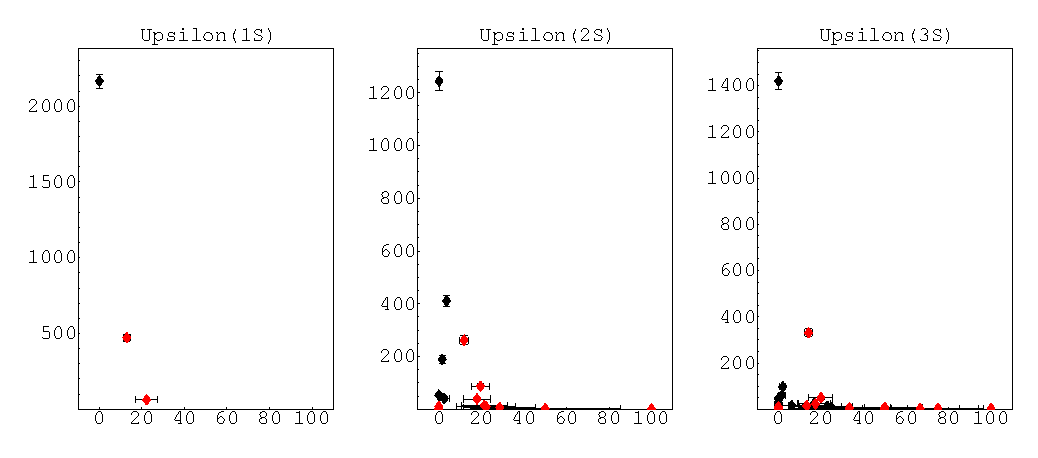
\includegraphics[width=\linewidth]{decayplot_mumu.pdf}
  \end{minipage} \\
  & \begin{minipage}{\linewidth}
    \begin{center}
      \vspace{-1.1 cm}
      Cut efficiency for each $\Upsilon \to \ldots \to X \mu^+\mu^-$ mode {\color{red} (red modes are from PHOTOS)}
    \end{center}
  \end{minipage}
\end{tabular}

\begin{center}
  \begin{tabular}{c | c c c c | c}
    \hline\hline
    & & & & & \\
    \begin{minipage}{3 cm} \begin{center} Resonance \end{center} \end{minipage} &
    \begin{minipage}{2 cm} \begin{center} Cut efficiency \end{center} \end{minipage} &
    \begin{minipage}{2 cm} \begin{center} Statisical Error \end{center} \end{minipage} &
    \begin{minipage}{4 cm} \begin{center} Variation with PDG mode uncertainties \end{center} \end{minipage} &
    \begin{minipage}{4 cm} \begin{center} Variation with fluctuating PHOTOS 30\% \end{center} \end{minipage} &
    \begin{minipage}{3 cm} \begin{center} Branching fraction to this set of modes \end{center} \end{minipage} \\
    & & & & & \\\hline
    & & & & & \\
    $\Upsilon(1S)$ & 2.81\% & $\pm$ 0.33 & $\pm$ 0 & $\pm$ 0.83 & 2.480\% $\pm$ 0.050 \\
    & & & & & \\
    $\Upsilon(2S)$ & 3.83\% & $\pm$ 0.51 & $\pm$ 0.076 & $\pm$ 0.82 & 2.04\% $\pm$ 0.14 \\
    & & & & & \\
    $\Upsilon(3S)$ & 4.37\% & $\pm$ 0.54 & $\pm$ 0.11 & $\pm$ 1.03 & 2.31\% $\pm$ 0.18 \\
    & & & & & \\\hline\hline
  \end{tabular}
\end{center}

\pagebreak

\begin{tabular}{p{0.02\linewidth} p{0.95\linewidth}}
  \begin{minipage}{\linewidth}
    \mbox{\hspace{0.3 cm} \begin{rotate}{90}
	\hspace{-3 cm} Occurrences in MC sample
    \end{rotate}}
  \end{minipage} &
  \begin{minipage}{\linewidth}
    \hspace{-0.5 cm} 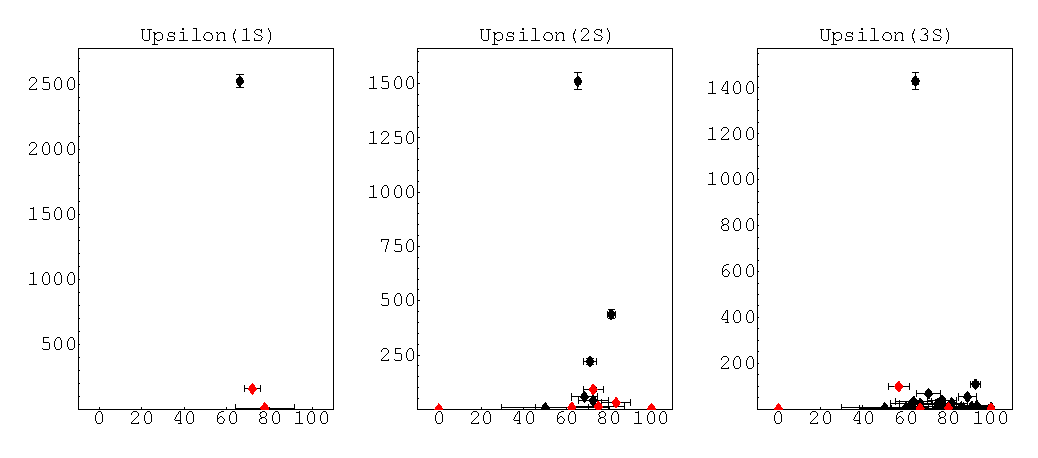
\includegraphics[width=\linewidth]{decayplot_tautau.pdf}
  \end{minipage} \\
  & \begin{minipage}{\linewidth}
    \begin{center}
      \vspace{-1.1 cm}
      Cut efficiency for each $\Upsilon \to \ldots \to X \tau^+\tau^-$ mode {\color{red} (red modes are from PHOTOS)}
    \end{center}
  \end{minipage}
\end{tabular}

\begin{center}
  \begin{tabular}{c | c c c c | c}
    \hline\hline
    & & & & & \\
    \begin{minipage}{3 cm} \begin{center} Resonance \end{center} \end{minipage} &
    \begin{minipage}{2 cm} \begin{center} Cut efficiency \end{center} \end{minipage} &
    \begin{minipage}{2 cm} \begin{center} Statisical Error \end{center} \end{minipage} &
    \begin{minipage}{4 cm} \begin{center} Variation with PDG mode uncertainties \end{center} \end{minipage} &
    \begin{minipage}{4 cm} \begin{center} Variation with fluctuating PHOTOS 30\% \end{center} \end{minipage} &
    \begin{minipage}{3 cm} \begin{center} Branching fraction to this set of modes \end{center} \end{minipage} \\
    & & & & & \\\hline
    & & & & & \\
    $\Upsilon(1S)$ & 66.5\% & $\pm$ 1.1 & $\pm$ 0 & $\pm$ 0.11 & 2.480\% $\pm$ 0.050 \\
    & & & & & \\
    $\Upsilon(2S)$ & 70.1\% & $\pm$ 1.2 & $\pm$ 0.32 & $\pm$ 0.092 & 2.04\% $\pm$ 0.14 \\
    & & & & & \\
    $\Upsilon(3S)$ & 67.8\% & $\pm$ 1.3 & $\pm$ 0.32 & $\pm$ 0.056 & 2.32\% $\pm$ 0.18 \\
    & & & & & \\\hline\hline
  \end{tabular}
\end{center}

\pagebreak

\begin{tabular}{p{0.02\linewidth} p{0.95\linewidth}}
  \begin{minipage}{\linewidth}
    \mbox{\hspace{0.3 cm} \begin{rotate}{90}
	\hspace{-3 cm} Occurrences in MC sample
    \end{rotate}}
  \end{minipage} &
  \begin{minipage}{\linewidth}
    \hspace{-0.5 cm} 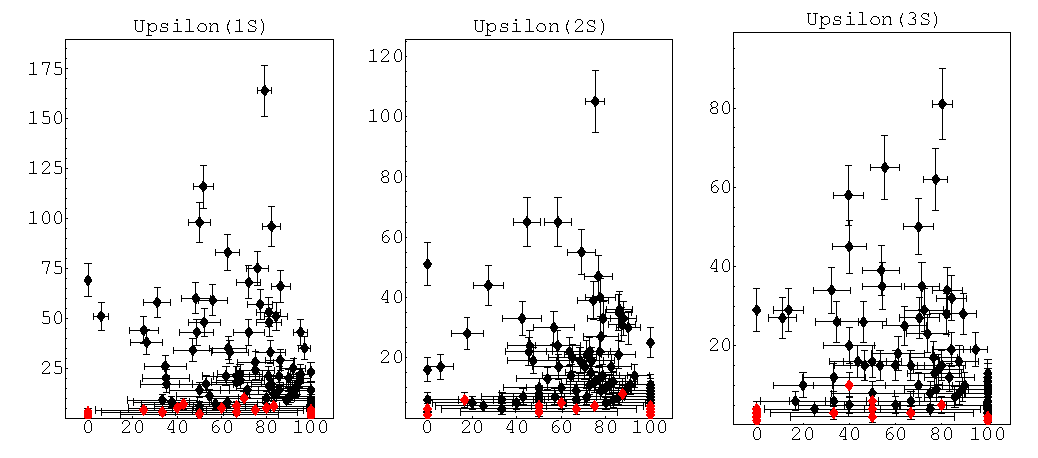
\includegraphics[width=\linewidth]{decayplot_taushape.pdf}
  \end{minipage} \\
  & \begin{minipage}{\linewidth}
    \begin{center}
      \vspace{-0.7 cm}
      Cut efficiency for each $\Upsilon \to \ldots \to X \tau^+\tau^-$, $\tau^+\tau^- \to Y$ mode {\color{red} (red modes are from PHOTOS)}
    \end{center}
  \end{minipage}
\end{tabular}
\begin{center}
  \begin{tabular}{c | c c c c | c}
    \hline\hline
    & & & & & \\
    \begin{minipage}{3 cm} \begin{center} Resonance \end{center} \end{minipage} &
    \begin{minipage}{2 cm} \begin{center} Cut efficiency \end{center} \end{minipage} &
    \begin{minipage}{2 cm} \begin{center} Statisical Error \end{center} \end{minipage} &
    \begin{minipage}{4 cm} \begin{center} Variation with PDG mode uncertainties \end{center} \end{minipage} &
    \begin{minipage}{4 cm} \begin{center} Variation with fluctuating PHOTOS 30\% \end{center} \end{minipage} &
    \begin{minipage}{3 cm} \begin{center} Branching fraction to this set of modes \end{center} \end{minipage} \\
    & & & & & \\\hline
    & & & & & \\
    $\Upsilon(1S)$ & 66.4\% & $\pm$ 1.1 & $\pm$ 0.088 & $\pm$ 0.12 & 2.481\% $\pm$ 0.050 \\
    & & & & & \\
    $\Upsilon(2S)$ & 70.5\% & $\pm$ 1.2 & $\pm$ 0.44 & $\pm$ 0.084 & 2.04\% $\pm$ 0.14 \\
    & & & & & \\
    $\Upsilon(3S)$ & 69.3\% & $\pm$ 1.4 & $\pm$ 0.52 & $\pm$ 0.091 & 2.32\% $\pm$ 0.17 \\
    & & & & & \\\hline\hline
  \end{tabular}
\end{center}

\pagebreak

\begin{tabular}{c c c c c c}
  \fbox{$\Upsilon(1S)$} & & & & & \vspace{-0.7 cm}\\
  & & $\begin{array}{c} \mbox{stat} \\ \overbrace{\mbox{\hspace{2 cm}}} \end{array}$ &
  $\begin{array}{c} \mbox{vary modes} \\ \overbrace{\mbox{\hspace{3 cm}}} \end{array}$ &
  $\begin{array}{c} \mbox{vary PHOTOS 30\%} \\ \overbrace{\mbox{\hspace{4 cm}}} \end{array}$ &
  $\begin{array}{c} \mbox{vary $\mathcal{B}(\frac{gg\gamma}{ggg})$ 33\%} \\ \overbrace{\mbox{\hspace{4 cm}}} \end{array}$ \\
  $\begin{array}{c} \mbox{(PDG $\mathcal{B}_{\mu\mu}$)} \\ \mbox{(Istvan's $\mathcal{B}_{\mu\mu}$)} \end{array}$ &
  \hspace{0.6 cm} $\begin{array}{c} \epsilon_\Upsilon = 0.9380 \\ \epsilon_\Upsilon = 0.9378 \end{array}$ &
  $\pm \mbox{ } 0.0008$ &
  $\pm \mbox{ } \begin{array}{c} 0.0009 \\ 0.0009 \end{array}$ &
  $\pm \mbox{ } 0.0039$ &
  $\pm \mbox{ } 0.0010$ \\
  & & & & & \\
  \fbox{$\Upsilon(1S) \to \mbox{hadrons}$} & & & & & \\
  & & & & & \\
  $\begin{array}{c} \mbox{(PDG $\mathcal{B}_{\mu\mu}$)} \\ \mbox{(Istvan's $\mathcal{B}_{\mu\mu}$)} \end{array}$ &
  $\begin{array}{c} \epsilon_{\Upsilon \to \mbox{\small had}} = 0.9942 \\ \epsilon_{\Upsilon \to \mbox{\small had}} = 0.9942 \end{array}$ &
  $\pm \mbox{ } 0.0003$ &
  $\pm \mbox{ } \begin{array}{c} 0 \\ 0 \end{array}$ &
  $\pm \mbox{ } 0$ &
  $\pm \mbox{ } 0.0011$ \\
  & & & & & \\
  \fbox{$\Upsilon(2S)$} & & & & & \\
  & & & & & \\
  $\begin{array}{c} \mbox{(PDG $\mathcal{B}_{\mu\mu}$)} \\ \mbox{(Istvan's $\mathcal{B}_{\mu\mu}$)} \end{array}$ &
  \hspace{0.6 cm} $\begin{array}{c} \epsilon_\Upsilon = 0.9500 \\ \epsilon_\Upsilon = 0.9365 \end{array}$ &
  $\pm \mbox{ } 0.0007$ &
  $\pm \mbox{ } \begin{array}{c} 0.0025 \\ 0.0011 \end{array}$ &
  $\pm \mbox{ } 0.0033$ &
  $\pm \mbox{ } 0.0008$ \\
  & & & & & \\
  \fbox{$\Upsilon(2S) \to \mbox{hadrons}$} & & & & & \\
  & & & & & \\
  $\begin{array}{c} \mbox{(PDG $\mathcal{B}_{\mu\mu}$)} \\ \mbox{(Istvan's $\mathcal{B}_{\mu\mu}$)} \end{array}$ &
  $\begin{array}{c} \epsilon_{\Upsilon \to \mbox{\small had}} = 0.9785 \\ \epsilon_{\Upsilon \to \mbox{\small had}} = 0.9781 \end{array}$ &
  $\pm \mbox{ } 0.0005$ &
  $\pm \mbox{ } \begin{array}{c} 0.0006 \\ 0.0006 \end{array}$ &
  $\pm \mbox{ } 0.0012$ &
  $\pm \mbox{ } 0.0009$ \\
  & & & & & \\
  \fbox{$\Upsilon(3S)$} & & & & & \\
  & & & & & \\
  $\begin{array}{c} \mbox{(PDG $\mathcal{B}_{\mu\mu}$)} \\ \mbox{(Istvan's $\mathcal{B}_{\mu\mu}$)} \end{array}$ &
  \hspace{0.6 cm} $\begin{array}{c} \epsilon_\Upsilon = 0.9448 \\ \epsilon_\Upsilon = 0.9325 \end{array}$ &
  $\pm \mbox{ } 0.0007$ &
  $\pm \mbox{ } \begin{array}{c} 0.0030 \\ 0.0017 \end{array}$ &
  $\pm \mbox{ } 0.0034$ &
  $\pm \mbox{ } 0.0009$ \\
  & & & & & \\
  \fbox{$\Upsilon(3S) \to \mbox{hadrons}$} & & & & & \\
  & & & & & \\
  $\begin{array}{c} \mbox{(PDG $\mathcal{B}_{\mu\mu}$)} \\ \mbox{(Istvan's $\mathcal{B}_{\mu\mu}$)} \end{array}$ &
  $\begin{array}{c} \epsilon_{\Upsilon \to \mbox{\small had}} = 0.9850 \\ \epsilon_{\Upsilon \to \mbox{\small had}} = 0.9829 \end{array}$ &
  $\pm \mbox{ } 0.0004$ &
  $\pm \mbox{ } \begin{array}{c} 0.0006 \\ 0.0006 \end{array}$ &
  $\pm \mbox{ } 0.0008$ &
  $\pm \mbox{ } 0.0008$ \\
\end{tabular}

\end{document}
